\newpage
\section{Solution Design}

The system we built is running on the Amazon Web Services (AWS) cloud. AWS provides all the necessary building tools and infrastructure to make such a distributed computing system possible as well as cost-effective. Other cloud providers have a similar and perfectly suitable offering, and AWS was simply a choice of personal taste.

The result of the project consists of the following three parts A, B, and C and can be seen in figure \ref{fig:system}.

\subsection{Information Retrieval}
This component downloads data from a suitable source (or many sources) to get daily information. We implemented it using serverless functions written in TypeScript leveraging cost benefits of AWS Lambda.

\subsection{Web application}
The application features several interactive visualizations on different COVID-19 related time series with several interactive aggregations that can be applied by the user. 

Types of time series:

\begin{itemize}
    \item Cases
    \item Tests
    \item Fatalities
    \item Vaccinations
    \item Test Positivity Rate
\end{itemize}

Aggregations (and combinations thereof):
\begin{itemize}
    \item By country
    \item Absolute, by 100,000, by 1,000,000 inhabitants, …
    \item Moving average by 14 days, 7 days, …
    \item Moving sum by 14 days, 7 days, ...
\end{itemize}

To provide an easy entry into the application, the main visualization is a world map showing the daily cases, or any other user-chosen metric (with possible aggregations), of the current day or an aggregation of the past.

Furthermore, the application provides the user with predictions computed based on historic data with the aggregations applied. So, they can predict if they will likely have to quarantine themselves upon return from their visit abroad e.g., because the 14-day moving average per 100,000 inhabitants is likely to be above 60 at the planned end of their trip or whatever metrics their government has issued.

It is made clear that these predictions are to be read with care, and they are not legally binding. It may also happen quite often that a prediction is totally unusable.

We implemented the backend with Java and Springboot. The frontend implementation uses Angular, Mapbox, d3.js, and Bootstrap.


\subsection{Prediction Engine}

The backend of the web application provides a prediction engine. Time series prediction is not an easy task and can deem as almost impossible in many cases if the data is irregular. Nonetheless, COVID-19 data often has regular patterns that can be discovered by learning algorithms. Most time series have a weekly seasonality and a clear trend.

The paper "Forecasting at Scale" \cite{b1} explains ways how to scale up the process of creating forecasting models and making it even approachable to people with little or no knowledge in fields like statistics or data science. The authors have also provided many of the methods packaged in a Python and R library called Prophet.

Our solution provides the user a prediction with a click of a button for their selected time series and settings. Based on the result, the user can then decide to start tweaking the hyper-parameters of the initial model and create a new model. Typical hyper-parameters in a model are change points, holidays and seasonality, and smoothing parameters. After the user of the application is happy with their model, they can then publish their predictions and share it with others.

These user-defined forecasting models are then explorable by all users and shareable by a URL.

We implemented this part using Python and Facebook's Prophet.

\begin{figure*}
\centerline{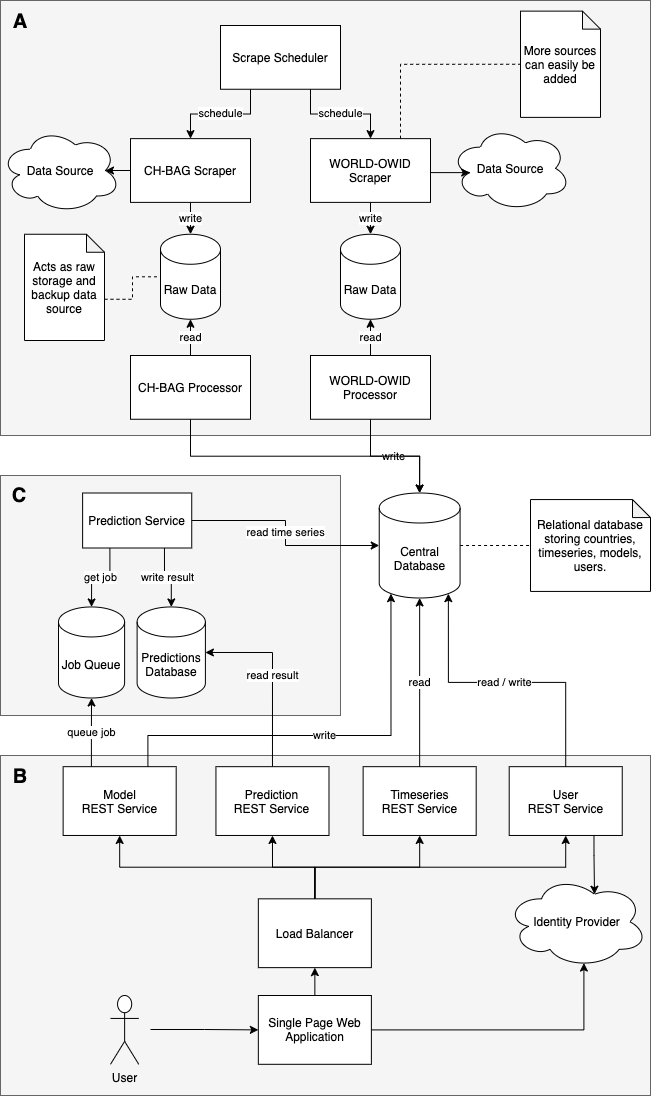
\includegraphics[scale=.5]{figs/system-diagram.png}}
\caption{Parts A, B, and C are grouped and consist each of several components. The central time series database is the way the three parts interact with the data. Part A: The information retrieval functions download the data from sources and import it into the database. Part B: The Web Application offers the end user a way to explore and interact with the data, as well as generate and retrieve predictions. Part C: The prediction engine listens for items in the job queue and executes them and stores the result back in a database, that the web application can then present to the user.}
\label{fig:system}
\end{figure*}
